%!TEX TS-program = pdflatex
%!TEX encoding = UTF-8 Unicode
\documentclass[a4paper]{book}
\sloppy
\usepackage{subfiles}
\usepackage[german, english]{babel}

% %%%%%%%%%%%%%%%%%%%%%%%%%%%%%%%%%%%%%%%%%%%%%%%%%%%%%%%%%%%%%%%%%%%%%
% preliminary version only, comment out if no longer needed
\usepackage{prelim2e}
\renewcommand{\PrelimText}{\sf\scriptsize --- INCOMPLETE DRAFT of \today ---}
\usepackage[colorinlistoftodos,bordercolor=orange,backgroundcolor=orange!20,linecolor=orange,textsize=scriptsize]{todonotes}
\setlength{\marginparwidth}{2.8cm}
% %%%%%%%%%%%%%%%%%%%%%%%%%%%%%%%%%%%%%%%%%%%%%%%%%%%%%%%%%%%%%%%%%%%%%

%\usepackage{caption2}
%\setcaptionwidth{1.0\textwidth}

\usepackage{wrapfig}
\usepackage[export]{adjustbox}
\usepackage[skip=2pt]{caption}
\usepackage{paralist}
\usepackage{bookmark}

\usepackage[]{graphicx}
\graphicspath{
	{image/}
	{figures/}
	{data/}
	{publications/AAG2012-Gridshells/}
	{publications/AAG2014-Periodic/final/images/}
	{publications/AAG2014-Periodic/final/}
}
\usepackage{color}

\usepackage{contour}
\contournumber{32}
\contourlength{0.1em}

\usepackage{amsmath}
\usepackage{amssymb}
\usepackage{amsthm}
\usepackage{mathtools}
\usepackage{gensymb}
\usepackage{accents}
\DeclarePairedDelimiter{\ceil}{\lceil}{\rceil}

\usepackage{url}
\usepackage{float}
\usepackage{colonequals}

\usepackage{enumitem}
\setlist{nolistsep}

\usepackage{listings}
\usepackage{pxfonts}
\lstset{language=JAVA}
\definecolor{middlegray}{rgb}{0.5,0.5,0.5}
\definecolor{lightgray}{rgb}{0.9,0.9,0.9}
\definecolor{orange}{rgb}{0.8,0.3,0.3}
\definecolor{yac}{rgb}{0.6,0.6,0.1}
\definecolor{javared}{rgb}{0.404,0,0.023}
\definecolor{javagreen}{rgb}{0.004,0.161,0.02}
\lstset{
   %backgroundcolor=\color{lightgray},
   basicstyle=\footnotesize\bfseries\ttfamily\color{javagreen},
   keywordstyle=\bfseries\ttfamily\color{javared},
   stringstyle=\normalfont\color{blue}\ttfamily,
   commentstyle=\color{middlegray}\ttfamily,
   emph={square},
   emphstyle=\color{blue}\texttt,
   emph={[2]root,base},
   emphstyle={[2]\color{yac}\texttt},
   showstringspaces=false,
   flexiblecolumns=false,
   tabsize=4,
   numbers=left,
   numberstyle=\tiny,
   numberblanklines=false,
   stepnumber=1,
   numbersep=10pt,
   xleftmargin=17pt,
   breaklines=true,
 }
\DeclareCaptionFormat{listing}{\rule{\dimexpr\textwidth+17pt\relax}{0.4pt}\vskip1pt#1#2#3}
\captionsetup[lstlisting]{format=listing,singlelinecheck=false, margin=0pt, labelsep=space,labelfont=bf}

% AAG2014
\usepackage[percent]{overpic}
%\usepackage{paralist}
\usepackage{xspace}
\usepackage{setspace}
\newcommand{\Epl}{E_{pl}}
\newcommand{\Ereg}{E_{reg}}
\newcommand{\VaryLab}{{\sc VaryLab}\xspace}
\newcommand{\nurbs}{{\sc nurbs}\xspace}

\usepackage{hyperref}
\usepackage[nottoc,numbib,notlof]{tocbibind}

% For Milnor's Lobachevsy function $\ML$
\usepackage[OT2,T1]{fontenc}
\newcommand{\ML}{\mbox{\fontencoding{OT2}\fontfamily{wncyr}\fontseries{m}\fontshape{n}\selectfont L}}

\usepackage[a4paper]{geometry}
%\usepackage{fancyhdr}
%\pagestyle{headings}
\setlength{\oddsidemargin}{15.5pt}
\setlength{\evensidemargin}{15.5pt}
\setlength{\parindent}{0pt}
\setlength{\parskip}{1ex}

\newtheorem{definition}{Definition}
\newtheorem{proposition}{Proposition}
\newtheorem{theorem}{Theorem}
\newtheorem*{remark*}{Remark}
\newtheorem*{remark}{Remark}
\newtheorem{example}{Example}
\newtheorem{problem}{Problem}[subsection]
\newtheorem{conjecture}{Conjecture}

\newcommand{\R}{\mathbb R}
\newcommand{\C}{\mathbb C}
\newcommand{\Z}{\mathbb Z}
\newcommand{\N}{\mathbb N}
\renewcommand{\S}{\mathbb S}
\newcommand{\Chat}{\hat{\mathbb C}}
\newcommand{\RP}{\R\mathrm{P}}
\newcommand{\T}{{\mathsf T}}
\newcommand{\cclass}{{\mathcal C}}
\newcommand{\Teich}{{\mathcal T}}
\newcommand{\PSL}{{\operatorname{\it PSL}}}
\newcommand{\ccr}{\operatorname{cr}}
\newcommand{\lcr}{\operatorname{lcr}}
\newcommand{\lmr}{\operatorname{lmr}}
\newcommand{\mean}{\operatorname{mean}}
\newcommand{\Eint}{E_{\mathit{int}}}
\newcommand{\Ebdy}{E_{\mathit{bdy}}}
\newcommand{\Vint}{V_{\mathit{int}}}
\newcommand{\Vbdy}{V_{\mathit{bdy}}}
\newcommand{\const}{\textit{const.}}
\newcommand{\grad}{\operatorname{grad}}
\newcommand{\hess}{\operatorname{hess}}
\newcommand{\degrees}{^{\circ}}
\newcommand{\re}{\operatorname{Re}}
\newcommand{\im}{\operatorname{Im}}
\newcommand{\arsinh}{\operatorname{arsinh}}
\newcommand{\arccot}{\operatorname{arccot}}
\newcommand{\Ehyp}{E^{\mathit{h}}}
\newcommand{\Vhyp}{V_{\mathit{h}}}
\newcommand{\Vhathyp}{\widehat{V}_{\mathit{h}}}
\newcommand{\vect}[1]{\accentset{\rightharpoonup}{#1}}
\newcommand{\alphat}{\tilde{\alpha}}
\newcommand{\betat}{\tilde{\beta}}
\newcommand{\ellt}{\tilde{\ell}}

\DeclareMathOperator{\sn}{sn}
\DeclareMathOperator{\cn}{cn}

\def\TReg{\textsuperscript{\textregistered} }

\title{Variational Methods for Discrete Surface Parameterization. Applications and Implementation.}
\author{Stefan Sechelmann}

\def\mainbibliography {
	\backmatter
	\setcounter{secnumdepth}{-1}
	\bibliographystyle{amsalpha}
	\bibliography{Thesis}
}
\def\subfilebibliography {
	\backmatter
	\setcounter{secnumdepth}{-1}
	\bibliographystyle{amsalpha}
	\bibliography{Thesis}
}
\def\subfilebibliographytwo {
	\backmatter
	\setcounter{secnumdepth}{-1}
	\bibliographystyle{amsalpha}
	\bibliography{Thesis}
}

\begin{document}
\def\subfilebibliography{}
\def\subfilebibliographytwo{}

\frontmatter
%\maketitle

\begin{titlepage}
\begin{center}
\large
{\Large\bf Variational Methods for Discrete Surface Parameterization. Applications and Implementation.}\\
\vspace{0.8cm}
vorgelegt von\\
%Dipl.-Math. techn. Stefan Sechelmann\\
Diplom-Technomathematiker Stefan Sechelmann\\
\vspace{0.8cm}
von der Fakult{\"a}t II - Mathematik und Naturwissenschaften\\
der Technischen Universit{\"a}t Berlin\\
zur Erlangung des akademischen Grades\\
\vspace{0.8cm}
Doktor der Naturwissenschaften\\
-- Dr. rer. nat. --\\
\vspace{0.8cm}
vorgelegte Dissertation\\
\vspace{0.8cm}
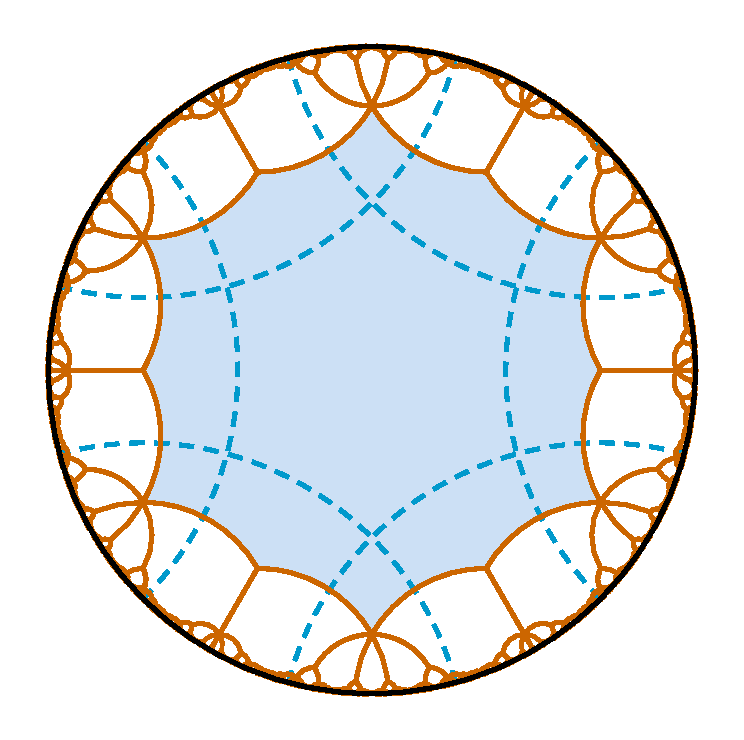
\includegraphics[width=0.4\linewidth]{introduction/title_lawson_cyclic.pdf}\\
\vspace{0.8cm}
Promotionsausschuss:\\
\vspace{0.3cm}
\begin{tabular}{rl}
Vorsitzende: & Prof. Dr. Gitta Kutyniok \\
Gutachter/Berichter: & Prof. Dr. Alexander I. Bobenko \\
& Prof. Dr. Max Wardetzky
\end{tabular}\\
\vspace{0.3cm}
Tag der wissenschaftlichen Aussprache: NN\\
\vspace{0.8cm}

Berlin, den {\selectlanguage{german}\today}\\
\vspace{0.3cm}
D 83
\end{center}
\end{titlepage}

\newpage

\tableofcontents
\newpage
%\listoffigures

\newpage
\mainmatter
\setcounter{secnumdepth}{-1}
\subfile{Chapter0_Introduction.tex}
\setcounter{secnumdepth}{2}
\part{Variational methods for discrete surface parameterization}
\label{part:uniformization}
\subfile{Chapter1_Uniformization.tex}
%\subfile{Chapter1_00_Preliminaries.tex}
%\subfile{Chapter1_01_Variational.tex}
%\subfile{Chapter2_Interpolation.tex}
%\subfile{Chapter1_02_DiscreteUniformization.tex}
%\subfile{Chapter1_03_Examples.tex}
\setcounter{part}{1}
\part{Applications}
\label{part:applications}
\subfile{Chapter2_PeriodicPanelization.tex}
\subfile{Chapter2_Quasiisothermic.tex}
\subfile{Chapter2_Tschebyscheff.tex}
\part{Implementation}
\label{part:implementation}
\subfile{Chapter3_JRworkspace.tex}
\subfile{Chapter3_Halfedge.tex}
\subfile{Chapter3_ConformalLab.tex}
\subfile{Chapter3_VaryLab.tex}

\newpage

\bookmarksetup{startatroot}
\mainbibliography

\backmatter
\appendix
\chapter{CD Content}
\label{chp:cd_content}

\chapter{Acknowledgements}

\end{document}
